\section{Results}

In this subsection we first describe the metrics used to evaluate the performance of the models on the skin lesion segmentation task. We then present the experimental environment setup and show the final results.

\subsection{Metrics}

Image segmentation models are mostly evaluated on the basis of how accurately they can predict each pixel. The prediction of the pixels can fall into one of four categories: true positive (TP), true negative (TN) or false positive (FP) and false negative (FN) respectively. The model’s performance is determined by the nature of its prediction and the aforementioned category it belongs to and the computed metrics derived therefrom.

The 2018 lesion segmentation challenge defines the \emph{Threshold Jaccard Index}, averaged over all images in the dataset, as the primary evaluation criteria where the threshold is set to 0.65 \citep{challenge-2018-codella}. The \emph{Jaccard Index}, also called Intersection over Union (IoU), is a method to quantify the percentage of overlap between the target mask (A) and our prediction output (B). It is formally defined as

\begin{equation}
  J(A, B) = \frac{|A \cup B|}{|A \cap B|}
\end{equation}

The Threshold Jaccard Index can then be calculated as

\begin{equation}
  TJ(A, B) = \begin{cases}
      J(A, B), & \text{if}\ J(A, B) \geq{0.65} \\
      0, & \text{otherwise}
    \end{cases}
\end{equation}

The Jaccard Index metric is closely related to the \emph{Dice Coefficient} which is often used as a loss function during training. We use the Dice Coefficient to calculate the area of overlap between the target mask and the predicted mask, defined as

\begin{equation}
  Dice = \frac{2TP}{2TP + FN + FP}
\end{equation}

Furthermore, \emph{accuracy} helps us to track the ratio between correctly predicted pixels over all pixels. For a given prediction, accuracy is defined as

\begin{equation}
  Accuracy = \frac{TP + TN}{TP + FP + TN + FN}
\end{equation}

Finally, \emph{sensitivity} measures the proportion of the correctly identified positives and is   calculated as

\begin{equation}
  Sensitivity = \frac{TP}{TP + FN}
\end{equation}

\emph{Specificity} tells us the proportion of the correctly identified negatives  and can be calculated as

\begin{equation}
  Specificity = \frac{TN}{TN + FP}
\end{equation}


\subsection{Experiments}

\subsubsection{Training Environment Setup}

All experiments were conducted using the same VM setup running Linux 18.04.1-Ubuntu (x86\_64). The underlying hardware contained 54 GiB physical memory, 64-bits Intel(R) Xeon(R) CPU E5-2690 v3 (2.60GHz) and NVIDIA Tesla K80 (8GK210GL, rev a1) GPU with 12 GiB physical memory.

\subsubsection{Approach}

We designed and ran 27 experiments in total. We used the following three machine learning frameworks as our experiment design guide:

\textbf{Ablative Analysis}: In order to determine the optimal image size for each model given the time and resources constraints, we performed ablation studies with input resolutions of 512x512 pixels, 2556x256 pixels, 192x256 pixels and 128x128 pixels. We also study the impact of transfer learning on the selected model architecture by adding or removing encoder weights pretrained on ImageNet. Furthermore, we study the effect of different encoder backbones in our encoder-decoder architectures.

\textbf{Approximation and estimation error}: We use the accuracy metrics to measure the performance of the models during training and inference time. We test different data preprocessing techniques like removing or adding hair to measure how much error is attributable to each method.

\textbf{Bias-variance diagnostic}: We use various regularization techniques like early stopping to understand the bias-variance trade-off and to prevent the models from overfitting in order to generalize well on unseen data. For final performance comparison, we report all previously defined metrics on an unseen test dataset.

\par
Table \ref{table:experiments} shows an overview over all experiment setups.

\begin{table*}[ht]
  \centering
  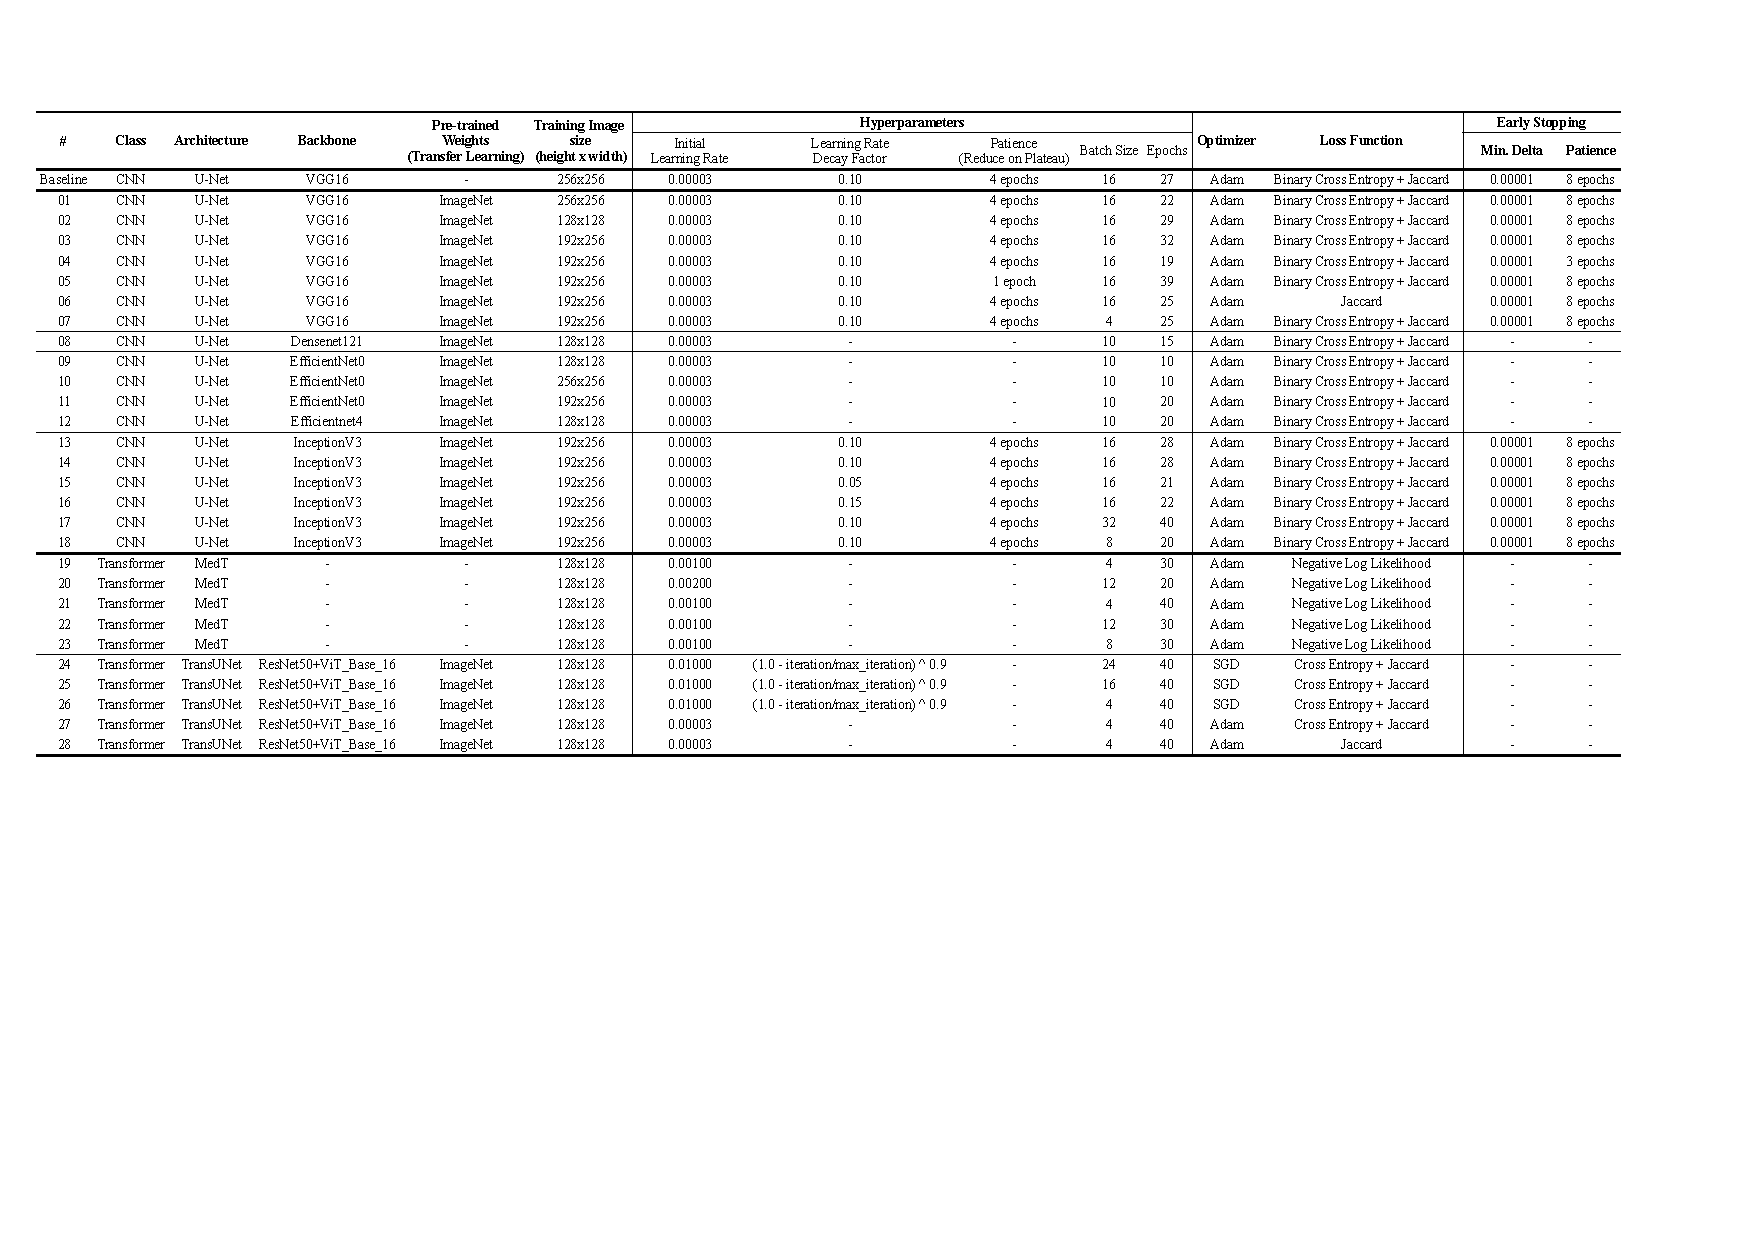
\includegraphics[width=\textwidth]{assets/experiments.pdf}
  \caption[Experiments]{Experimental model configurations with hyperparameter settings, optimizer, loss function and early stopping setup. First row corresponds to the baseline model.}
  \label{table:experiments}
\end{table*}

\par
Table \ref{table:results} summarizes all experiment results.

\begin{table*}[ht]
  \centering
  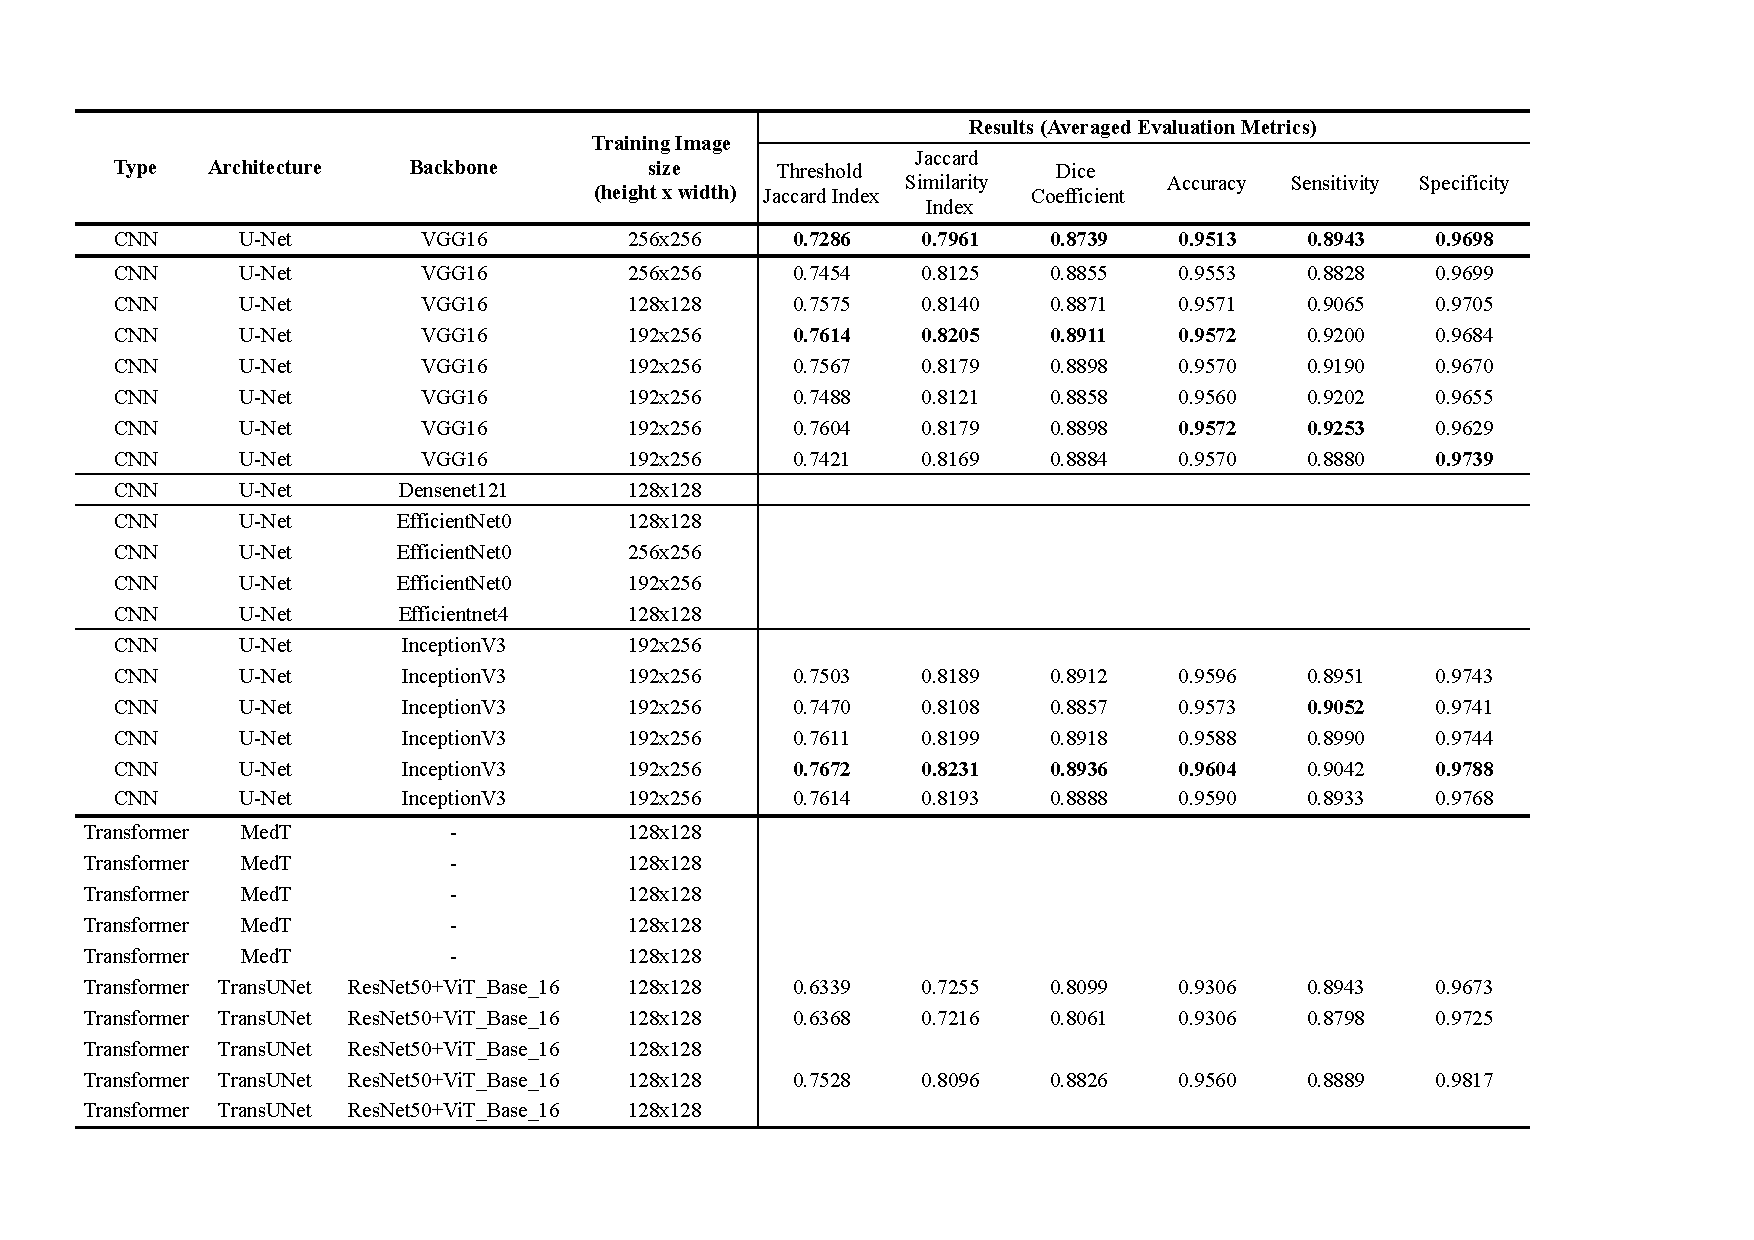
\includegraphics[width=\textwidth]{assets/results.pdf}
  \caption[Results]{Model flavors with corresponding type, architecture, input image sizes and final results as reported on unseen test dataset. First row corresponds to the baseline model.}
  \label{table:results}
\end{table*}

% \begin{itemize}
%   \item Describe all Machine Learning Theory techniques used to evaluate the success of the model.
%   \item Describe how results compare to previous research.
% \end{itemize}
